\documentclass{article} % This command is used to set the type of document you are working on such as an article, book, or presenation

\usepackage{geometry} % This package allows the editing of the page layout
\usepackage{amsmath}  % This package allows the use of a large range of mathematical formula, commands, and symbols
\usepackage{graphicx}  % This package allows the importing of images
\usepackage{tikz} % This package allows the creation of graphics and diagrams
\usepackage{pdfpages}
\usetikzlibrary{calc} % This library allows the use of advanced coordinate calculations

\newcommand{\maketitletwo}[2][]{\begin{center}
        \Large{\textbf{Assignment 3}
            
            Foundations of Audio Signal Processing} % Name of course here
        \vspace{5pt}
        
        \normalsize{Caspar Wiswesser, Vitezslav Kula, Prasun Dutta, Arash Astanboos % Your name here
        }
        \vspace{15pt}
        
\end{center}}
\begin{document}
    \maketitletwo[1]  % Optional argument is assignment number
    %Keep a blank space between maketitletwo and \question[1]
    
    \section*{Exercise 3.1}
    \subsection*{a)}

    \begin{align*}
        cos(\alpha) &= \frac{1}{2} (2\cos\alpha) = \frac{1}{2} (2\cos\alpha + i \sin\alpha - i \sin\alpha) \\
        &= \frac{1}{2} (cos\alpha + i \sin\alpha + \cos(-\alpha) + i \sin(-\alpha)) \\
        &= \frac{1}{2} (e^{i \alpha} + e^{-i \alpha})
    \end{align*}

    \subsection*{b)}
    
    \begin{align*}
        \sin(\alpha + \beta) &= \frac{i \sin(\alpha + \beta)}{i} = \frac{i \sin(\alpha + \beta) + \cos(\alpha + \beta) - \cos(\alpha + \beta)}{i} \\
        &= \frac{e^{\alpha + \beta} - \cos(\alpha + \beta)}{i} = \frac{e^\alpha e^\beta - \cos(\alpha + \beta)}{i} \\
        &= \frac{1}{i} ((\cos\alpha + i \sin\alpha)(\cos\beta + i \sin\beta) - \cos(\alpha + \beta)) \\
        &= \frac{1}{i} (\cos\alpha \cos\beta + \cos \alpha ~ i \sin\beta + i \sin\alpha \cos\beta + i^2 \sin\alpha \sin\beta - \cos(\alpha + \beta)) \\
        &= \cos \alpha \sin \beta + \cos \beta \sin \alpha + \frac{1}{i} (\cos \alpha \cos \beta - \sin \alpha \sin \beta - \cos(\alpha + \beta)) \\
        &= \cos \alpha \sin \beta + \cos \beta \sin \alpha + \frac{1}{i} (\cos(\alpha + \beta) - \cos(\alpha + \beta)) \\
        &= \cos \alpha \sin \beta + \cos \beta \sin \alpha
    \end{align*}

    \subsection*{c)}

    \begin{align*}
        \sin(\alpha)^2 + \cos(\alpha)^2 &= \sin(\alpha)^2 + i \sin(\alpha)\cos(\alpha) - i \sin(\alpha)\cos(\alpha) + \cos(\alpha)^2 \\
        &= (\cos\alpha + i \sin\alpha)(\cos\alpha - i \sin\alpha) \\
        &= e^{i \alpha} e^{-i \alpha} = e^{i \alpha - i \alpha} = e^0 = 1
    \end{align*}

    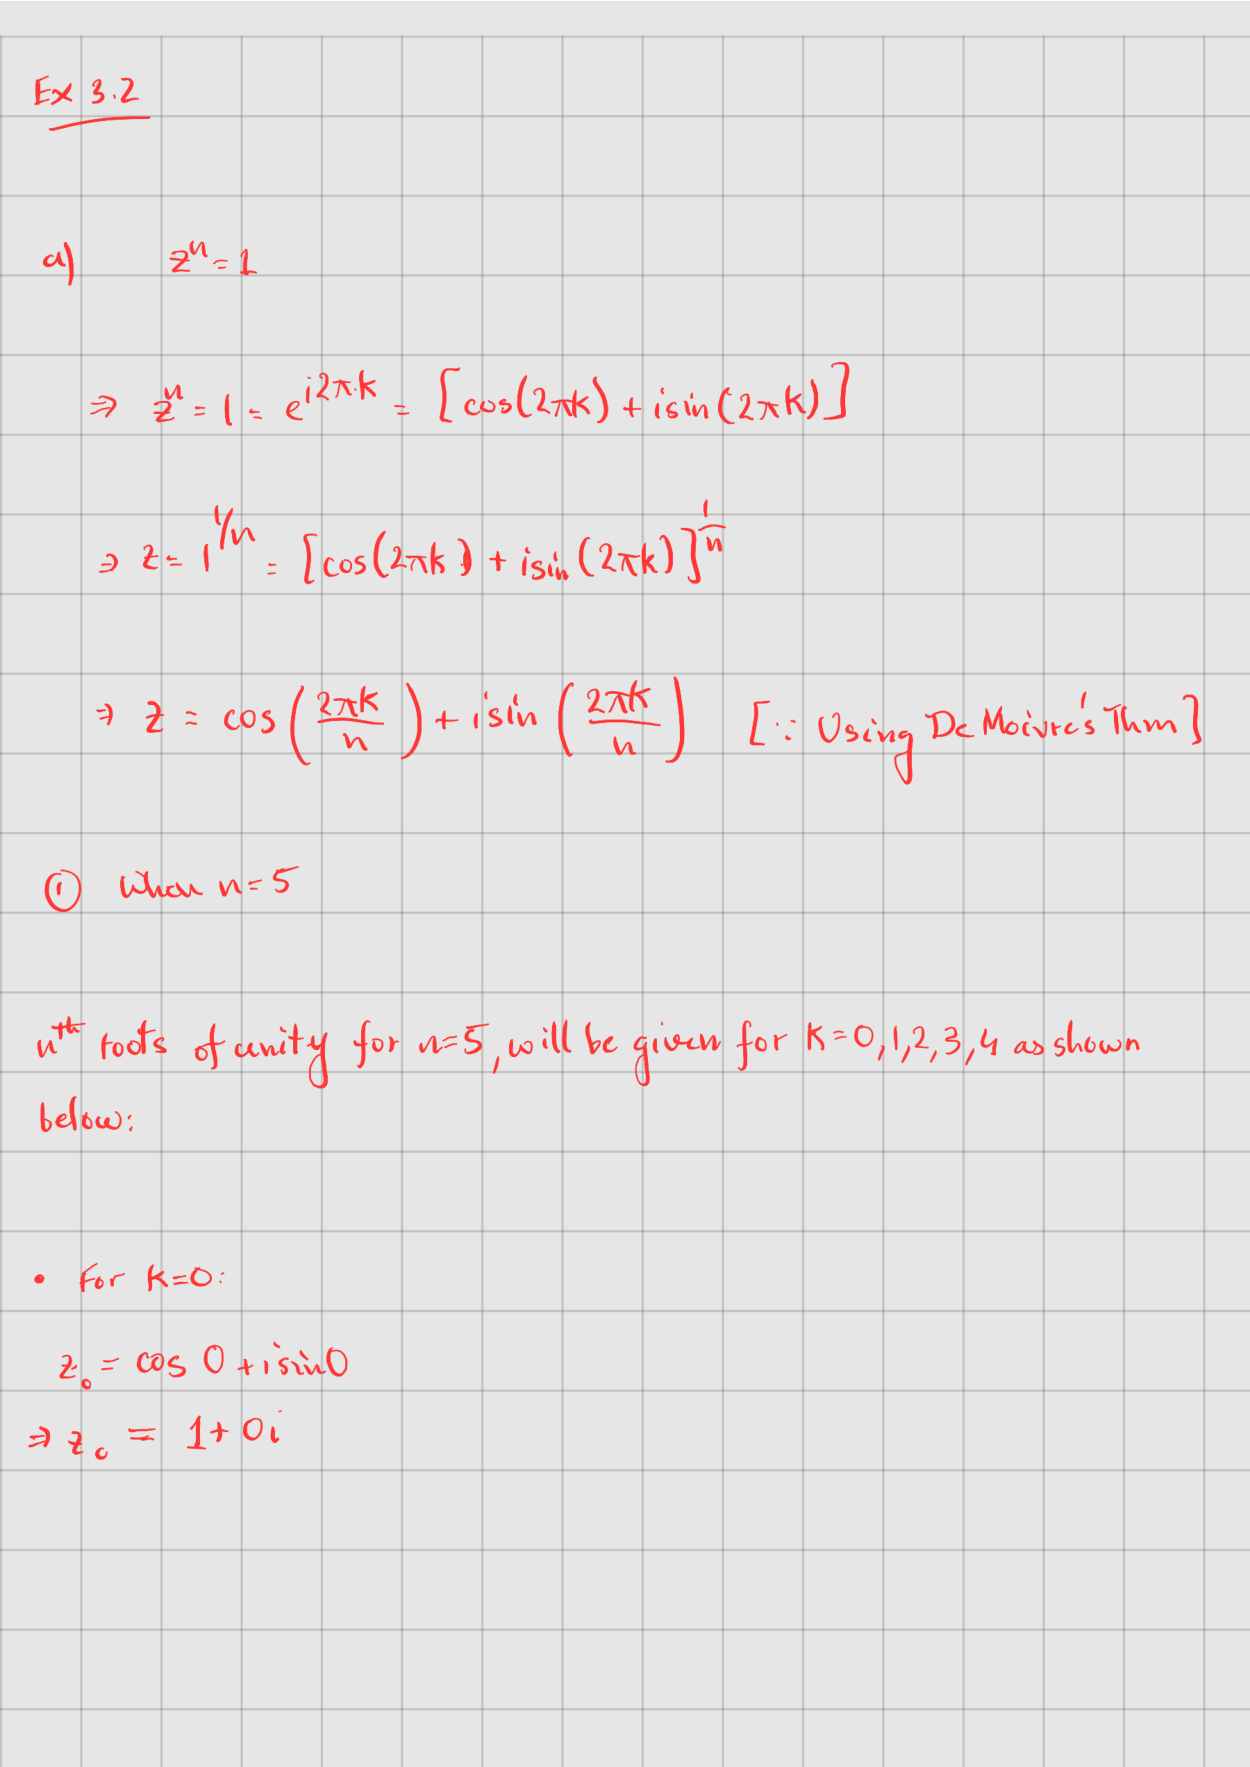
\includepdf[pages={-}]{Ex_3_Part_2.pdf}
\end{document}-